\documentclass[10pt]{IEEEtran}
\usepackage[utf8]{inputenc}
\usepackage{graphicx}
\usepackage{float}
\usepackage{amsmath}
\usepackage{algorithm2e}
\usepackage{listings}
\interdisplaylinepenalty=2500
\bibliographystyle{ieeetr}

\lstset{frame=tb,
language=C,
aboveskip=3mm,
belowskip=3mm,
showstringspaces=false,
columns=flexible,
basicstyle={\small\ttfamily},
numbers=none,
breaklines=true,
breakatwhitespace=true,
tabsize=3
}

\title{Método Sarrus Paralelo Extendido a Matrices de Tamaño Mayor a 3}
\author{
  \IEEEauthorblockN{Blancarte Lopez Jorge,
  Lievana Poy Erick and
  Ocampo Alvarez Jose Alvaro}\\
  \IEEEauthorblockA{Facultad de Ciencias de la Computación,
  Benemérita Universidad Autónoma de Puebla
  Email:jorge.blancarte@alumno.buap.mx,
  erick.lievanap@alumno.buap.mx,
  jose.ocampo@alumno.buap.mx}}

\begin{document}

\maketitle

\begin{abstract}
  En este trabajo se analiza la eficiencia de la programación paralela con el uso de las librerias de OpenMPI para el cálculo de la regla extendida de Sarrus para matrices mayores a 3x3. Se compararan los tiempos del algoritmo secuencial y el algoritmo paralelo.
\end{abstract}

\begin{IEEEkeywords}
  Algoritmo, Paralelo, Secuencial, Tiempo, MPI, Procesos.
\end{IEEEkeywords}

\section{Introducción}

Para el presente se tiene por objetivo aplicar y crear un escenario comparativo de la ejecución de la regla de Sarrus extendida de forma secuencial contra su forma paralelizada para eso se implementaron en el lenguaje de programación C con el uso de las librerias de OpenMPI, la regla de Sarrus extendida.

\section{Antecedentes}

\subsection{Regla de Sarrus Extendida}
La regla de Sarrus es un método fácil para memorizar y calcular un determinante 3×3. Recibe su nombre del matemático francés Pierre Frédéric Sarrus, que la introdujo en el artículo \textit{Nouvelles méthodes pour la résolution des équations}, publicado en Estrasburgo en 1833.

\begin{equation}
  \begin{bmatrix}
    a_{11} & a_{12} & a_{13} \\
    a_{21} & a_{22} & a_{23} \\
    a_{31} & a_{32} & a_{33}
  \end{bmatrix}
\end{equation}

Dada la anterior matriz de $3x3$ se puede calcular su determinante de la siguiente forma:

\begin{equation}
  \begin{aligned}
    det =
    &a_{11} a_{22} a_{33} +
    a_{21} a_{32} a_{13} +
    a_{31} a_{12} a_{23}\\
    -
    &a_{13} a_{22} a_{31} -
    a_{23} a_{32} a_{11} -
    a_{33} a_{12} a_{21}
  \end{aligned}
\end{equation}

Se puede llegar al mismo resultado al repetir las dos primeras filas de la matriz debajo de la misma de manera que queden cinco filas. Después sumar los productos de las diagonales descendentes y sustraer los productos de las diagonales ascendentes.

\begin{figure}
  \centering
  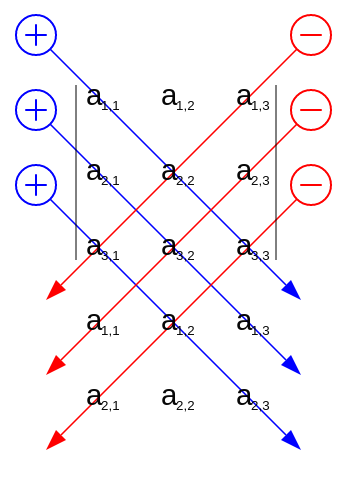
\includegraphics[height=2in]{reglaSarrus.png}
  \caption{La regla de Sarrús: las diagonales azules se suman y las diagonales rojas se restan.}
  \label{fig:reglaSarrus}
\end{figure}

Para poder expander la regla de Sarrus a matrices de mayor tamaño, debemos primero comprender como es que se generan las diagonales. Empecemos con una matriz general de nxn.

\begin{equation}
  \begin{bmatrix}
    a_{11} & a_{12} & \cdots & a_{1n} \\
    a_{21} & a_{22} & \cdots & a_{2n} \\
    \vdots & \vdots & \ddots & \vdots \\
    a_{n1} & a_{n2} & \cdots & a_{nn}
  \end{bmatrix}
\end{equation}

A partir de esta matriz podemos deducir que las diagonales descendientes seran las mostradas en la ecuación \ref{eq:diagPos}, con esto podemos crear un algoritmo para poder obtener las diagonales descendientes. Como podemos observar el indice de las columnas siempre va desde $0$ hasta $n$, mientras que el indice de las filas va incrementando por $1$ en cada diagonal y cuando llega al limite de las filas, se reinicia a $0$.

\begin{equation}
  \label{eq:diagPos}
  \begin{aligned}
    &a_{00}a_{11}a_{22}\cdots a_{nn}\\
    &a_{10}a_{21}a_{32}\cdots a_{n(n-1)}a_{0n}\\
    &\vdots \\
    &a_{n0}a_{01}a_{12}\cdots a_{(n-2)(n-1)}a_{(n-1)n}
  \end{aligned}
\end{equation}

\begin{algorithm}
  \label{algoDes}
  \SetAlgoLined
  \KwResult{Calcular las diagonales descendentes}
  \For{i = 0; i\textless n; i++}{
    diagonalActual = 1\;
    \For{j = 0; j\textless n; j++}{
      \eIf{i + j\textgreater = n}{
        diagonalActual *= $a_{(i+j)j}$\;
      }{
        diagonalActual *= $a_{((i+j)-n)j}$\;
      }
    }
    totalDiagonalesAscendentes = diagonalActual\;
  }
  \caption{Algoritmo para calcular las diagonales descendientes}
\end{algorithm}

Por lo que basandonos en la manera general para recorrer matrices, podemos crear el algoritmo \ref{algoDes}, seran 2 ciclos \textit{for} que recorreran la matriz. La primera diagonal siempre la diagonal donde ambos indices son iguales es decir $a_{kk}$ por lo que cuando $i = 0$ como $i + j$ no puede ser mayor que $n$ entonces $a_{(i+j)j} = a_{jj}$. Para casos donde $i > 0$ podemos observar que habra un punto donde $i + j >= n$ y en esta situacion se usara $a_{((i+j)-n)j}$ y para el caso donde $i + j = n$ se reiniciara el indice de las filas a $0$ lo que hace posible calcular las diagonales descendientes sin repetir renglones de la matriz.

Para el caso de las diagonales ascendentes, tenemos que las diagonales generadas tendran las forma presentada en la ecuación \ref{eq:diagNeg}. Podemos observar ahora el indice de las columnas va de $n$ a $0$ mientras que el de las filas se mantiene con la misma logica que el de las diagonales ascendentes, por que lo que es posible modificar el algoritmo \ref{algoFinal} para tambien calcular las diagonales descendientes para tambien calcular las diagonales ascendentes.

\begin{equation}
  \label{eq:diagNeg}
  \begin{aligned}
    &a_{0n}a_{1(n-1)}a_{2(n-2)}\cdots a_{n0}\\
    &a_{1n}a_{2(n-1)}a_{3(n-2)}\cdots a_{(n-1)1}a_{n0}\\
    &\vdots \\
    &a_{nn}a_{0(n-1)}a_{1(n-2)}\cdots a_{(n-2)1}a_{(n-1)0}
  \end{aligned}
\end{equation}

\begin{algorithm}
  \label{algoFinal}
  \SetAlgoLined
  \KwResult{Calcular todas las diagonales}
  \For{i = 0; i\textless n; i++}{
    diagonalActualPositiva = 1\;
    diagonalActualNegativa = 1\;
    \For{j = 0; j\textless n; j++}{
      \eIf{i + j\textgreater = n}{
        diagonalActualPositiva *= $a_{(i+j)j}$\;
        diagonalActualNegativa *= $a_{(i+j)(n-j)}$\;
      }{
        diagonalActualPositiva *= $a_{((i+j)-n)j}$\;
        diagonalActualNegativa *= $a_{((i+j)-n)(n-j)}$\;
      }
    }
    totalPositivas += diagonalActualPositiva\;
    totalNegativas += diagonalActualNegativa\;
  }
  \caption{Algoritmo para calcular todas las diagonales}
\end{algorithm}

\subsection{MPI}
MPI (iniciales de Message Passing Interface) es una especificación para programación de paso de mensajes, que proporciona una librería de funciones para C, C++ y Fortran que son empleadas en los programas para comunicar datos y portable, especificada por consenso por el MPI Forum, con unas 40 organizaciones participantes, como modelo que permita desarrollar programas que puedan ser migrados a diferentes computadores paralelos.

Definido conjuntamente por proveedores de hardware y de software, OpenMP es un modelo de programación portable y escalable que proporciona a los programadores una interfaz simple y flexible para el desarrollo de aplicaciones paralelas, para plataformas que van desde las computadoras de escritorio hasta supercomputadoras.

Para este problema desarrollamos un programa en el lenguaje de programación C usando openMPI con un tipo de comunicacion de punto a punto lineal esto significa que los procesos envian la información procesada al siguiente proceso en el rank asi como en la figura \ref{fig:lineal}. Al final es el ultimo proceso en el rank el que junta toda la información y la muestra o guarda.

\begin{figure}
  \centering
  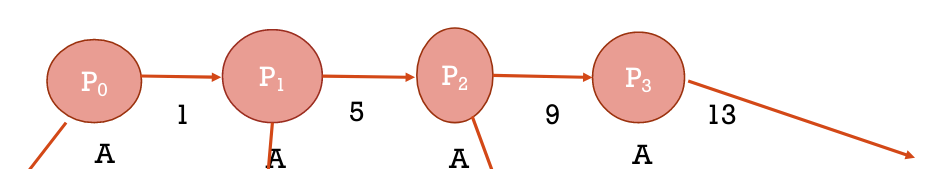
\includegraphics[width=0.8\linewidth]{lineal.png}
  \caption{Comunicación lineal entre 4 procesos}%
  \label{fig:lineal}
\end{figure}

\section{Desarrollo}
Para desarrollar este experimento es necesario implementar el algoritmo \ref{algoFinal} en lenguaje C de forma que cada proceso pueda calcular cierta cantidad de diagonales y aportarlas a la suma de las diagonales descendentes y las diagonales ascendentes respectivamente. Asi mismo para representar la comunicación de punto a punto lineal es necesario que los procesos se comuniquen entre si y envien los resultados de sus ejecuciones. Al final del reporte se anexara la totalidad del codigo.

\subsection{Implementación de Sarrus Paralelo}
Como mencionamos debemos permitir que cada proceso calcule solo un cierto rango de diagonales, como cada diagonal inicia con el primer elemento de una fila, entonces hay tantas diagonales como filas tiene las matriz, por lo que al dividir $n$ entre el numero total de procesos obtendremos el tamaño de los rangos, y al multiplicarlos por el rank de cada proceso podemos obtener el inicio de cada rango. Para esto se implemento el codigo del listing \ref{lst:sarrus} en C.

\begin{lstlisting}[caption={Implementacion de Sarrus Paralelo},label={lst:sarrus}]
void sarrusPorRank(int rank,long double DiagArray[2],int matriz[orden][orden]){
  int from = (rank * orden)/numeroDeRanks;
  int to = ((rank+1) * orden)/numeroDeRanks;
  long double temporalNegativa;
  long double temporalPositiva;
  int i,j;
  int fila;
  DiagArray[0] = 0;
  DiagArray[1] = 0;

  printf("computing rank \%d (from row \%d to \%d)\n", rank, from, to-1);
  for(i = from; i < to; i++){
    temporalNegativa = 1;
    temporalPositiva = 1;
    for(j = 0; j < orden; j++){
      fila = i+j;
      if(fila >= orden){
        fila -= orden;
      }
      temporalPositiva *= matriz[fila][j];
      temporalNegativa *= matriz[fila][(orden-1)-j];
    }
    DiagArray[0] += temporalNegativa;
    DiagArray[1] += temporalPositiva;
  }
  printf("finished rank \%d\n", rank);
}
\end{lstlisting}

Como podemos ver en el Listing \ref{lst:sarrus} se muestra la función que hara el cálculo de las Diagonales de Sarrus, esta función recibe la matriz de la cual se desean calcular las diagonales, el numero de rank del proceso que la llama y finalmente recibe un vector de tamaño 2 donde se guardaran los resultados.

La primera parte de la función utiliza el rank para calcular el rango de diagonales que los procesos van a calcular, esto para dividir la matriz de forma uniforme entre los procesos.

La siguiente parte hace la declaración de las variables de apoyo que se usaran para el calculo de las diagonales. Puesto que se calculan las diagonales descendentes y las diagonales ascendentes al mismo tiempo entonces debemos crear variables para ambos casos.

En la siguiente parte anunciamos que proceso esta haciendo el calculo e implementamos el algoritmo \ref{algoFinal}, para paralelizarlo solo vamos a recorrer el rango de diagonales calculado en la primera parte. Para ello nuestra variable $i$ solo debera recorrer desde el valor de la variable $from$ hasta el valor de la variable $to$. Y se guardan los resultados en el vector de resulstados $DiagArray$ siendo el indice $0$ los resultados de las diagonales ascendentes y el indice $1$ los resultados de las diagonales descendentes. Finalmente el proceso reporta su finalización.

\subsection{Implentación Comunicación Punto a Punto}
Como se ve en la figura \ref{fig:lineal} los procesos desde el mas bajo hasta el penultimo, envian sus resultados al proceso que les sigue, es decir el proceso $k$ envia su información al proceso $k+1$. Para esto MPI ofrece las funciones \textit{MPI\textunderscore Recv} y \textit{MPI\textunderscore Send} que permiten enviar información entre los procesos. Con estas funciones podemos implementar el codigo dle listing \ref{lst:lineal} en C.

\begin{lstlisting}[caption={Implementacion de Comunicación Lineal},label={lst:lineal}]
if(rank == 0){
  sarrusPorRank(rank,tmp,A);
  Diagonales[0] = tmp[0];
  Diagonales[1] = tmp[1];
  if(numeroDeRanks > 1)
  MPI_Send(Diagonales, 2, MPI_LONG_DOUBLE, rank+1, tag, MPI_COMM_WORLD);
  MPI_Send(A, orden*orden, MPI_INT, rank+1, tag, MPI_COMM_WORLD);
}
if(rank == numeroDeRanks - 1){
  if(numeroDeRanks > 1){
    MPI_Recv(Diagonales, 2, MPI_LONG_DOUBLE, rank-1, tag, MPI_COMM_WORLD, &status);
    MPI_Recv(A, orden*orden, MPI_INT, rank-1, tag, MPI_COMM_WORLD, &status);
    sarrusPorRank(rank,tmp,A);
    Diagonales[0] += tmp[0];
    Diagonales[1] += tmp[1];
  }
  end = MPI_Wtime();
  if(orden < 21) imprimirMatriz(A);
  printf("Sarrus calculation done.\n\n");
  printf("Pos final: \%Lf rank: \%d\n",Diagonales[1],rank);
  printf("Neg final: \%Lf rank: \%d\n",Diagonales[0],rank);
  printf("Determinante = \%Lf rank: \%d\n",Diagonales[1]-Diagonales[0],rank);
  printf("Pos final: \%Le rank: \%d\n",Diagonales[1],rank);
  printf("Neg final: \%Le rank: \%d\n",Diagonales[0],rank);
  printf("Determinante = \%Le rank: \%d\n",Diagonales[1]-Diagonales[0],rank);
  printf("Tiempo: \%lf rank: \%d\n",end-start,rank);
  printf("\n");

  FILE *file1;
  file1 = fopen("datosTiempo.txt","a+");
  if(file1 != NULL){
    fprintf(file1,"\%lf\n",end - start);
  }
  fflush(file1);
  fclose(file1);
}
if(rank != 0 && rank != numeroDeRanks - 1){
  MPI_Recv(Diagonales, 2, MPI_LONG_DOUBLE, rank-1, tag, MPI_COMM_WORLD, &status);
  MPI_Recv(A, orden*orden, MPI_INT, rank-1, tag, MPI_COMM_WORLD, &status);
  sarrusPorRank(rank,tmp,A);
  Diagonales[0] += tmp[0];
  Diagonales[1] += tmp[1];
  MPI_Send(Diagonales, 2, MPI_LONG_DOUBLE, rank+1, tag, MPI_COMM_WORLD);
  MPI_Send(A, orden*orden, MPI_INT, rank+1, tag, MPI_COMM_WORLD);
}
\end{lstlisting}

En el listing \ref{lst:lineal} que pertenece a la función main del programa, lo primero que se puede notar es que se checa que si el rank del proceso es 0, esto es importante ya que cada programa MPI tendra por lo menos un proceso cuyo rank sera 0. En este caso el proceso con rank 0, llamara a la función vista en el listing \ref{lst:sarrus} le pasara su rank que es cero, un array $tmp$ que es donde guardaran los resultados temporalmente y finalmente la matriz $A$. Una vez ejecutada la función los resultados guardados en el array $tmp$ seran guardados en el array \textit{Diagonales} que almanaceran los resultados definitivos. Despues si hay mas de 1 proceso, entonces el proceso con rank 0 enviara el array \textit{Diagonales} y la matriz al siguiente proceso. En caso de ser solo el proceso con rank 0 no se enviara ninguna información.

Despues se checara si el proceso es el ultimo proceso, en caso de ser el último proceso se checara si hay mas de un proceso, esto para el caso donde solo haya un solo proceso, en este caso el procesos con rank 0 es el primer y el ultimo proceso, en caso de que sea asi y solo hay un proceso no se recibira nada de otro proceso y tampoco hay que volver a llamar la función de listing \ref{lst:sarrus} y por lo tanto no hay cambio a los resultados por lo que se puede pasar directamente al manejor de resultados. En caso de que si haya mas de un proceso, entonces se recibe la información otorgada por el penultimo proceso y el ultimo procesos hace sus ejecuciones correspondientes al llamar la funcion del listing \ref{lst:sarrus} pasando su rank, el array $tmp$ y la matriz A, despues calcula los resultados finales al sumarle al array \textit{Diagonales} los resultados guardados temporalmente en el array $tmp$.

Para mostrar los resultados el ultimo proceso, los mostrara en pantalla con la funcion \textit{printf} de manera normal asi como en notación cientifica esto debido a que se generan números muy grandes hasta del orden $10^{1400}$ aproximadamente.

De igual forma el ultimo proceso es responsable de guardar los distintos tiempos de ejecución a un archivo de texto llamado \textit{datosTiempo.txt}

Finalmente aquellos procesos que no tengan rank $0$ o sean el ultimo rank, primero recibiran la matriz y los resultados del procesos con rank anterior, ejecutaran la función vista en el listing \ref{lst:sarrus} guardaran los resultados en el array \textit{Diagonales} y pasaran la matriz y el array \textit{Diagonales} al siguiente proceso.

\section{Resultados}
Es importante resaltar que los resultados obtenidos como vimos se componen de números grandes del orden de $10^{1400}$ esto debido a los tamaños de las matrices. Sin embargo en este trabajo no nos concentraremos en los resultados si no en los tiempos de ejecución. Para ello habran 2 categorias una donde se comparan los tiempo de ejecución con distintos números de procesos,

\subsection{Ejecución con distintos procesos}

\section{Conclusiones}

\section{Referencias}
{[1]} Fox G., M. Johnson, G. Lyzenga, S. Otto, J. Salmon, and D. Walker, Solving Problems on Concurrent Processors, Vol. I, Prentice Hall, Englewood Cliffs, New Jersey, 1988.

\end{document}
